% ================= 1. INTRODUCTION =================
\section{Introduction}

\subsection{Background \& Problem Statement}
\label{sec:background}

The Cubli is a reaction-wheel inverted pendulum: a cube-shaped platform that balances on an edge or a corner using only internal actuation, with no external supports or contact forces beyond the single line or point of contact with the ground. The concept was introduced by the Institute for Dynamic Systems and Control (IDSC) at ETH Zurich \cite{gajamohan2012cubli, gajamohan2013cubli}, whose original prototype ($15\times15\times15$~cm) mounts one brushless DC motor and flywheel on each of three orthogonal faces. Commanding a change in wheel speed produces, by conservation of angular momentum, an equal and opposite reaction torque on the cube body; braking a wheel abruptly transfers its stored angular momentum to the body in a near-impulsive event, which is what allows the cube to \emph{jump up} from resting on a face into a balance on an edge or corner.

Dynamically, the system is an \emph{underactuated}, nonlinear, unstable-equilibrium control problem: three actuators (the wheels) must stabilise a body with more degrees of freedom than actuated inputs, about equilibria (edge and corner balance) that are open-loop unstable and increasingly coupled across axes as the contact geometry shrinks from a line (edge) to a point (corner). This is structurally the same problem as the classical inverted pendulum, extended from a single rotational axis to a fully three-dimensional, momentum-exchange-actuated body — which is why the Cubli has become a standard benchmark platform in the controls community over the past decade.

The problem this project addresses is therefore twofold: (i) derive and validate a dynamic model and controller capable of stabilising this underactuated system about its unstable equilibria and driving it through commanded reorientations, and (ii) realise this in hardware as a modular, largely parametric design, since final actuator and sensor specifications are not yet confirmed at the time of writing. The target capability set, in order of increasing difficulty, is edge balance, corner balance, controlled rotation, and walking (Section~\ref{sec:objectives}).

No single subsystem is exotic, but each sits close to a physical bound, and the bounds are coupled: relieving one tightens another. Four constraints drive the design, and sizing is therefore treated as the first engineering activity rather than a detail settled once parts arrive.

\begin{itemize}
    \item \textbf{The jump-up has no energy margin.} The required per-wheel inertia scales as $M L^{3/2}$ (Section~\ref{sec:jumpup_target}), so mass added anywhere demands a larger wheel, and the wheel is itself part of $M$. Sizing is a fixed-point iteration, not a one-pass calculation.
    \item \textbf{Braking torque fights the structure.} Momentum accumulated over seconds of spin-up is shed in tens of milliseconds, through one shaft, hub and motor mount --- the parts the mass budget wants thin. The structural load case is set by the manoeuvre that proves the machine works.
    \item \textbf{Sensing, not the control law, sets the balancing limit.} Gyroscope bias drifts, and the accelerometer --- the only absolute tilt reference --- is corrupted by vibration the controller itself generates. Wheel balance is therefore an estimation requirement, not a mechanical nicety.
    \item \textbf{The plant is nonlinear and constrained.} Corner balancing does not decouple into three single-axis problems: the axes are coupled through the contact point and the inertia tensor. The actuators saturate in both torque and speed, so stored momentum must be actively managed. Linearising about upright is adequate for balancing and inadequate for anything more \cite{muehlebach2017cubli}.
\end{itemize}

\subsection{Purpose, Application \& Mission Context}
\label{sec:application}

The Cubli problem is a useful tool for teaching students about control engineering, mechanical engineering, electrical engineering, and programming, and it is thus presented as a kit that teaches the concepts used in spacecraft attitude determination systems. 

The Cubli is not presented here as a balancing novelty but as a terrestrial, gravity-loaded demonstrator of \textbf{momentum-exchange attitude control} — the same physical mechanism that governs how real spacecraft point themselves. Nearly every three-axis-stabilised satellite holds and changes its attitude using reaction wheels: flywheels whose commanded speed change produces a reaction torque on the spacecraft body, exactly as in the Cubli. Spacecraft typically carry three or four such wheels (often in a pyramidal arrangement for redundancy) — directly analogous to the Cubli's three orthogonal wheels — and this reaction-wheel approach is the standard for CubeSats and small satellites in particular, making the Cubli representative of a real, currently-flown hardware class rather than an idealized toy problem.

% \label{sec:tradeoff}
% Reaction wheels are the actuator choice made here, and the alternative is worth stating explicitly because it is the standard smallsat comparison. Since this is a proof-of-concept demonstration of the control loop, a system actuated with orthogonal reaction wheels is well-suited to represent principles applicable to smallsat ADCS: the momentum-exchange actuation principle and closed-loop control architecture are the same as those used on real spacecraft, even though the Cubli's dynamics (balancing against gravity) differ from a satellite's free-fall attitude control problem. Reaction wheels are also structurally simpler and require less specialised hardware than control moment gyros, which offer higher torque density but at the cost of gimbal mechanisms and more complex control software --- complexity that is typically only justified on larger spacecraft. For a low-cost, resource-limited project, a reaction-wheel Cubli therefore demonstrates the core actuation and control principles of smallsat ADCS in a practical and relevant way.

Framed as an Attitude Determination and Control System (ADCS) problem, the Cubli's core behaviours map directly onto a spacecraft's day-to-day pointing task:

\begin{itemize}
    \item \textbf{Edge / corner balance} $\rightarrow$ regulation to a commanded reference attitude and disturbance rejection --- holding a pointing setpoint against perturbations.
    \item \textbf{Controlled rotation} $\rightarrow$ a slew manoeuvre: reference tracking to a new commanded attitude, exactly as a satellite re-aims a payload or antenna.
    \item \textbf{Jump / walk} $\rightarrow$ momentum-exchange hopping mobility, flight-proven on small bodies where wheeled traction is impossible (Figure~\ref{fig:momentum_exchange_applications}). Walking, as a sequence of controlled directional hops, extends single-hop capabilities and represents an active research frontier (Section~\ref{sec:objectives}).
\end{itemize}

% Panels are cropped to a common 4:3 aspect ratio so the three source images
% (originally 1.10, 1.78 and 2.00 wide) render at identical size. Trim lengths
% are in pt and derived from each file's natural size as reported by graphicx,
% not from its pixel grid -- the two differ per image because of the embedded DPI.
\begin{figure}[htbp]
\centering
\begin{minipage}[t]{0.32\textwidth}
  \centering
  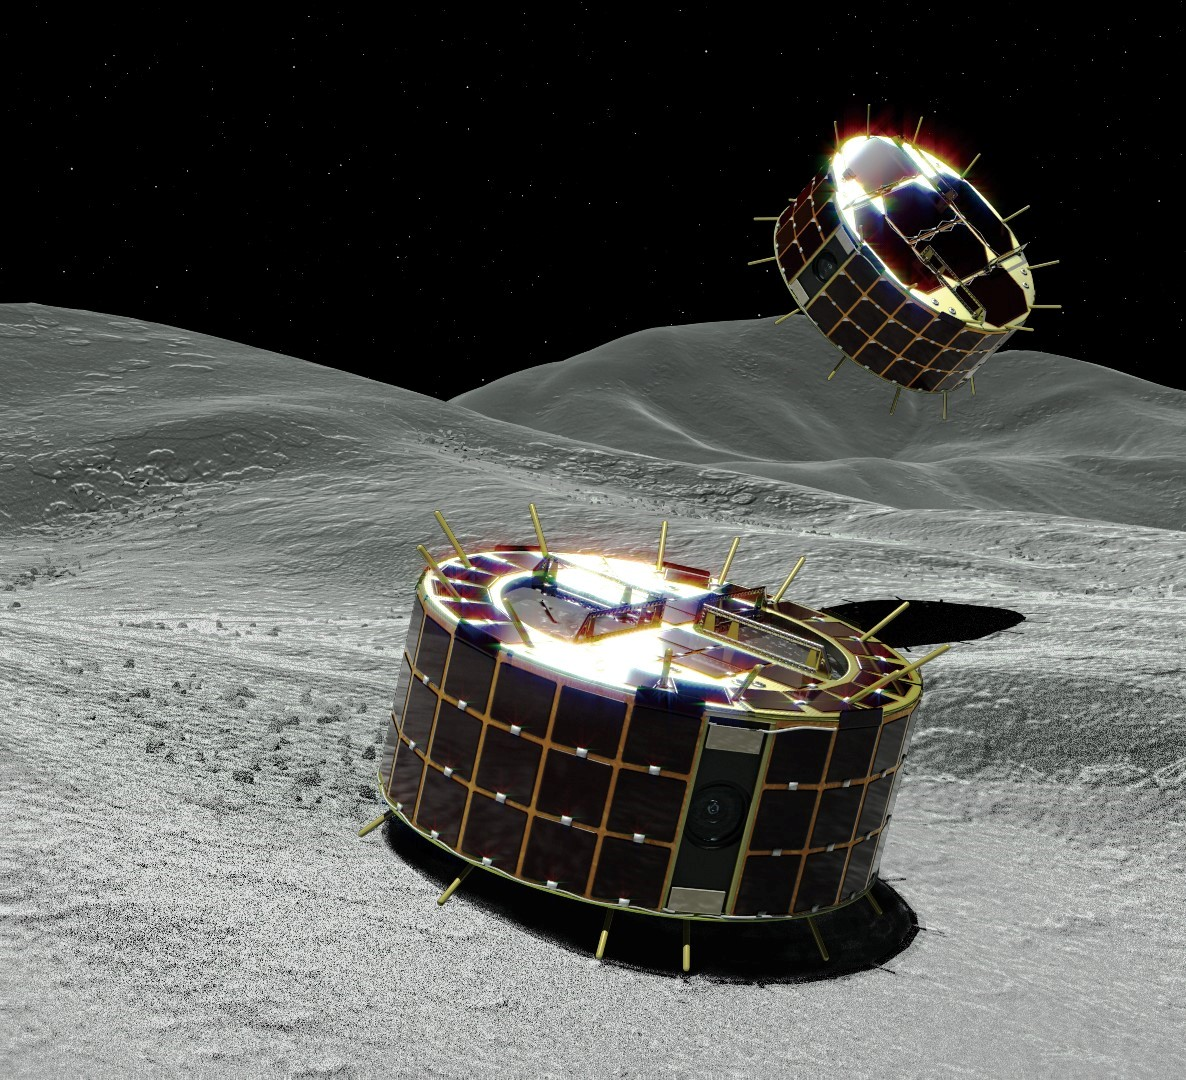
\includegraphics[trim=0 22.94pt 0 22.94pt,clip,width=\linewidth]{images/MINERVA-II1.jpg}\\[2pt]
  {\small (a) MINERVA-II1}
\end{minipage}\hfill
\begin{minipage}[t]{0.32\textwidth}
  \centering
  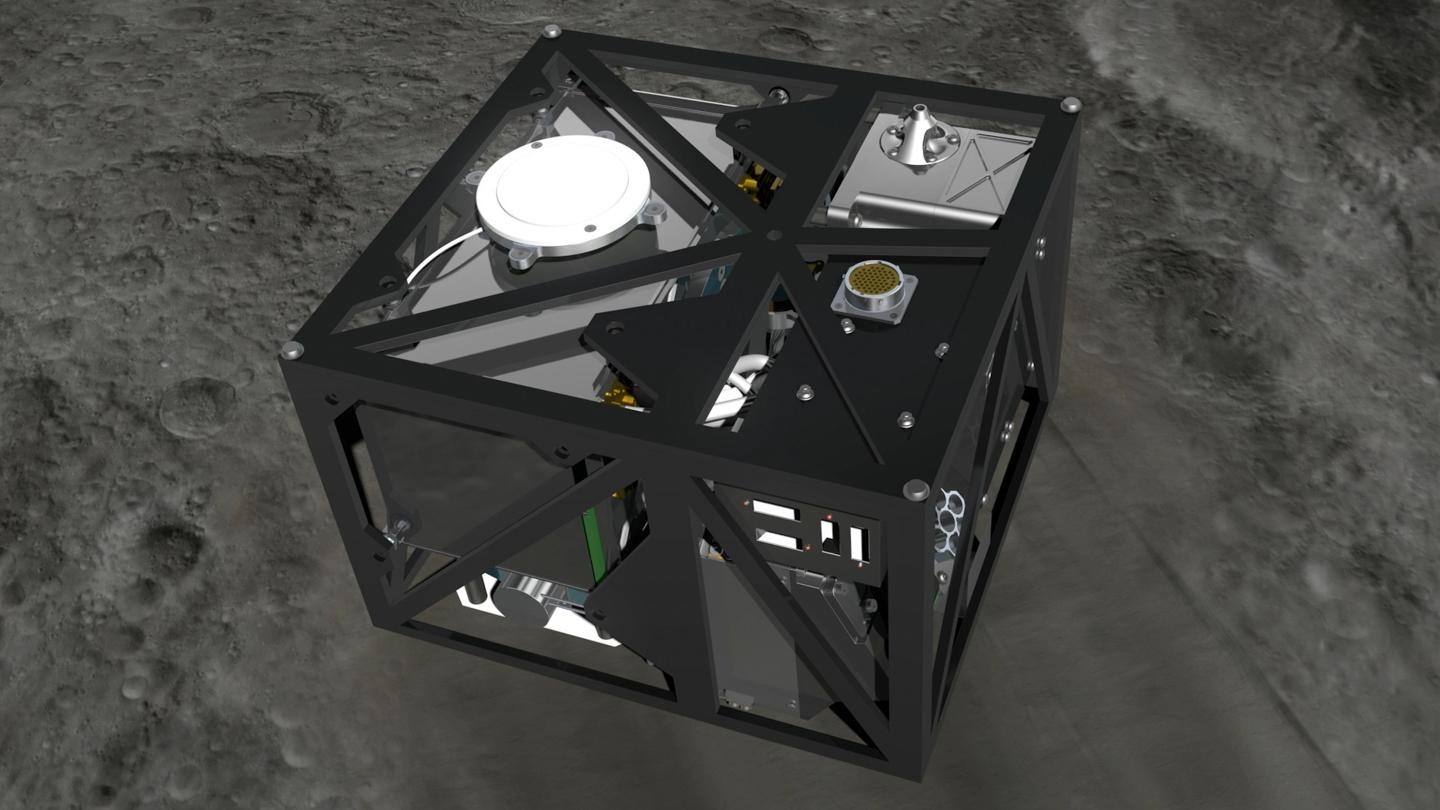
\includegraphics[trim=180.67pt 0 180.67pt 0,clip,width=\linewidth]{images/mascot_lander.jpeg}\\[2pt]
  {\small (b) MASCOT}
\end{minipage}\hfill
\begin{minipage}[t]{0.32\textwidth}
  \centering
  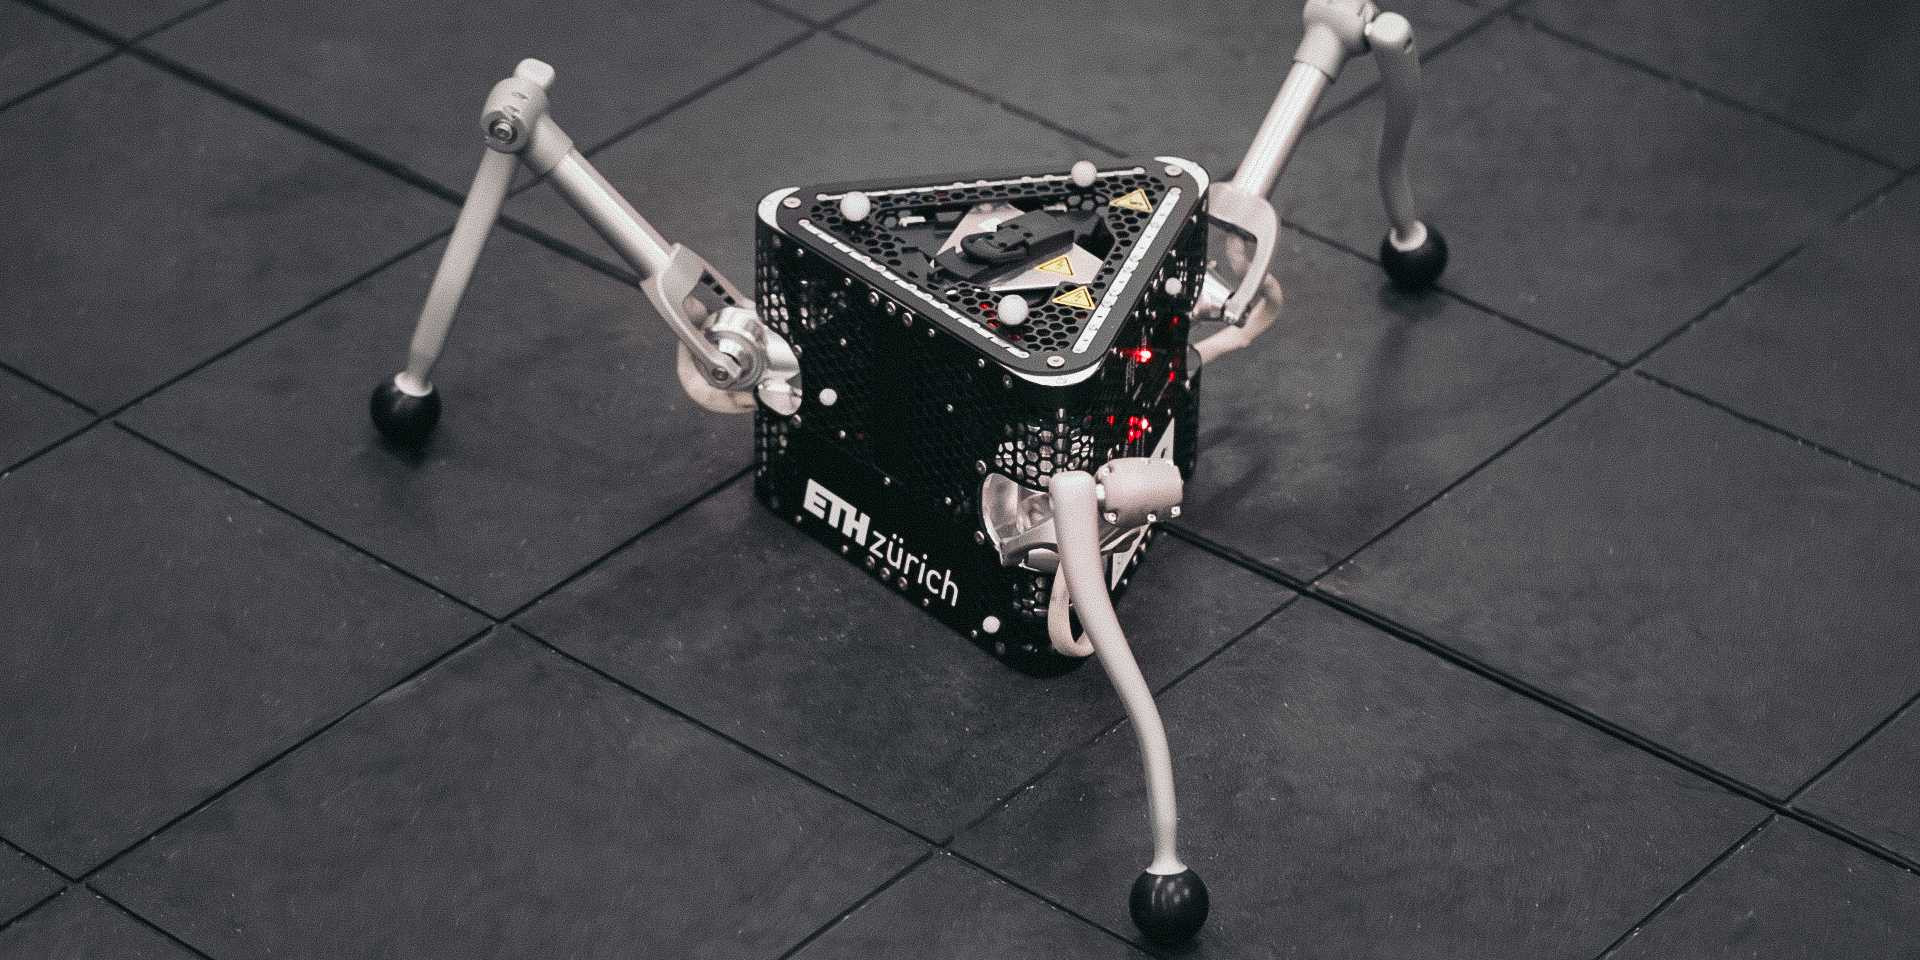
\includegraphics[trim=321.2pt 0 321.2pt 0,clip,width=\linewidth]{images/spacehopper.jpg}\\[2pt]
  {\small (c) SpaceHopper}
\end{minipage}
\caption[Flight and research platforms using momentum-exchange mobility]{Momentum-exchange actuation in flight and research hardware: (a) JAXA's MINERVA-II1 rovers \cite{yoshimitsu1999minerva} and (b) the MASCOT lander \cite{ho2017mascot}, deployed by Hayabusa2 onto asteroid Ryugu (2018), hop across the surface and self-right by spinning up and braking an internal flywheel or eccentric mass; (c) ETH Zurich's SpaceHopper \cite{spiridonov2024spacehopper} extends this principle to controlled, directional hopping in low gravity.}
\label{fig:momentum_exchange_applications}
\end{figure}

The subsystem exercised here is therefore the one a spacecraft uses for pointing: momentum-exchange attitude control under actuator saturation, with desaturation, on an underactuated body whose inertia is imperfectly known. Under gravity the destabilising torque never relents, so an inadequate controller falls over immediately and unambiguously --- the demonstration is self-evaluating, which a free-fall attitude testbed is not.

The nominal Cubli problem was solved a decade ago on precisely manufactured hardware \cite{gajamohan2012cubli, gajamohan2013cubli, muehlebach2017cubli}; reproducing it is an engineering exercise, and this document claims no more. A commodity build is adopted for three reasons. It can be crashed repeatedly, so the controller can be tested at its limits; its loose tolerances, imperfectly balanced wheels and drifting IMU supply the parameter uncertainty that robust control methods are intended to tolerate; and a fixed motor, print volume and budget constrain the sizing, since a marginal design cannot be rescued by specifying a larger component. The last of these motivates the adjustable ballast scheme of Section~\ref{sec:rw_sizing}.

\subsection{Objectives}
\label{sec:objectives}

Each project objective imposes a required capability. The mapping below keeps
every requirement traceable from motivation to capability, and is what the
sizing and control work below must be shown to satisfy.

\begin{table}[htbp]
\centering
\caption[Objective-to-requirement traceability]{Objective-to-requirement traceability.}
\label{tab:traceability}
\begin{tabular}{lp{0.65\textwidth}}
\toprule
Objective & Required capability \\
\midrule
Edge balance        & The system must actively maintain dynamic stability and regulate its posture about a single line-contact equilibrium position. \\[0.5em]
Corner balance      & The system must maintain multi-axis closed-loop balance and attitude control around a highly unstable point-contact equilibrium. \\[0.5em]
Controlled rotation & The controller must accurately track dynamic reference trajectories to execute smooth slew maneuvers between distinct equilibrium states. \\[0.5em]
Walking (stretch)   & The system must execute a sequential series of dynamic jump-up maneuvers and rapidly re-stabilize itself upon each landing impact. \\
\bottomrule
\end{tabular}
\end{table}

These map one-to-one onto the applications of Section~\ref{sec:application}: (1)–(2) demonstrate pointing regulation and disturbance rejection of increasing difficulty; (3) demonstrates slew/reference-tracking; (4) demonstrates momentum-exchange mobility of the kind flown on Hayabusa 2. Milestones (1)–(3) are treated as committed deliverables for this design; walking (4) is scoped as the stretch objective, contingent on hardware confirmation and the jump-up feasibility check (angular momentum required to tip the cube vs.\ available motor/wheel torque), to be resolved once final components are known.